\section{Research Thrust 1: Device and Circuit-level Exploration for
Emerging NVMs (PI: Li, Co-PI: Xie)}

\subsection{Task C-1: Device models and circuit analysis methodology}



\subsection{Task C-2: Explore novel circuit techniques for NVM}
\label{C2-Circuit}

The advent of novel devices have introduced a number of new design issues. In general, the requirements for all the memories are similar, \emph{e.g.} fast speed, high density, affordable yield, low power, \emph{etc}. However, depending on the applications and process development stage, the primary concerns for different technologies could be quite different. Furthermore, the different technologies may need different solutions for the same issue, which mainly rely on the specific device characteristics. Our task is to investigate the corresponding circuit design issues and explore novel circuit techniques for the emerging NVMs.

\subsubsection{Task C-2.1: STT-RAM -- process variation-tolerant design}
In STT-RAM design, there are two main constrains from MTJ device characteristics. (i) The difference between two resistance states of MTJ ($R_H$ $\&$ $R_L$) is fairly small: $\Delta$R=$R_H-R_L$ $\approx$ $1000\Omega$ at 45nm technology node~\cite{Li09}. (ii) The large MTJ resistance variation $\sigma_R$ is another challenge. For example, MTJ resistance increases exponentially with the thickness of oxide barrier between two magnetic layers. It was reported in~\cite{Tehrani00} that MTJ resistance increases by 8\% when the thickness of oxide barrier changes from 14${\AA}$ to 14.1${\AA}$. Moreover, the MTJ resistance variation will be aggravated by the further reduction of oxide barrier thickness in scaled technologies. Besides oxide barrier thickness, MTJ resistance is also significantly affected by the large MTJ geometry variations.

The small $\Delta$R and the large $\sigma_R$ could lead to the false detection of the stored value. For example, in a conventional voltage sensing scheme, read current $I_R$ is sent to the STT-RAM cell and generates bitline (BL) voltage $V_{BL,L}=I_R\cdot(R_L+R_{TR})$ or $V_{BL,H}=I_R\cdot(R_H+R_{TR})$, when the MTJ is at the low resistance state and the high resistance state, respectively~\cite{Li09}. Here, $R_{TR}$ is the resistance of NMOS transistor. By comparing the BL voltage to a reference voltage $V_{REF}$ between $V_{BL,L}$ and $V_{BL,H}$, the MTJ resistance state can be readout. Usually a $V_{REF}$ is shared by multiple STT-RAM bits, hence it needs to satisfy: $\max(V_{BL,L})<V_{REF}<\min(V_{BL,H})$. Here, $\max(V_{BL,L})$ and $\min(V_{BL,H})$ denote the maximal $V_{BL,L}$ and the minimal $V_{BL,H}$ generated by all involved STT-RAM bits, respectively. Unfortunately, \textbf{\emph{$\max(V_{BL,L})<\min(V_{BL,H})$ may not be always true when the bit-to-bit variation of MTJ resistance is large.}} New read-out scheme is required to overcome the STT-RAM processor variation and improve chip yield.

\paragraph{A nondestructive self-reference read scheme.} We propose a nondestructive self-reference methodology to reduce read failures in STT-RAM design. The basic idea is to compare the stored data in a memory cell with a reference value written to the same cell. By limiting the comparison within one single STT-RAM cell, the impact of bit-to-bit variation of MTJ resistance can be avoided. Previously some \emph{destructive} self-reference schemes were used in toggle-mode MRAM design~\cite{Tanizaki06,Jeong03}. We also successfully utilized it in STT-RAM design~\cite{Li:147723,Chen:147727}. We call these schemes ``destructive'' because the original value in memory cell is wiped out when writing the reference value into MTJ, and has to be recovered at the end of the read operation. Obviously it prolongs read latency and introduces reliability issue.

\begin{wrapfigure}{r}{0.45\textwidth}\centering \centering
\vspace{-18pt}
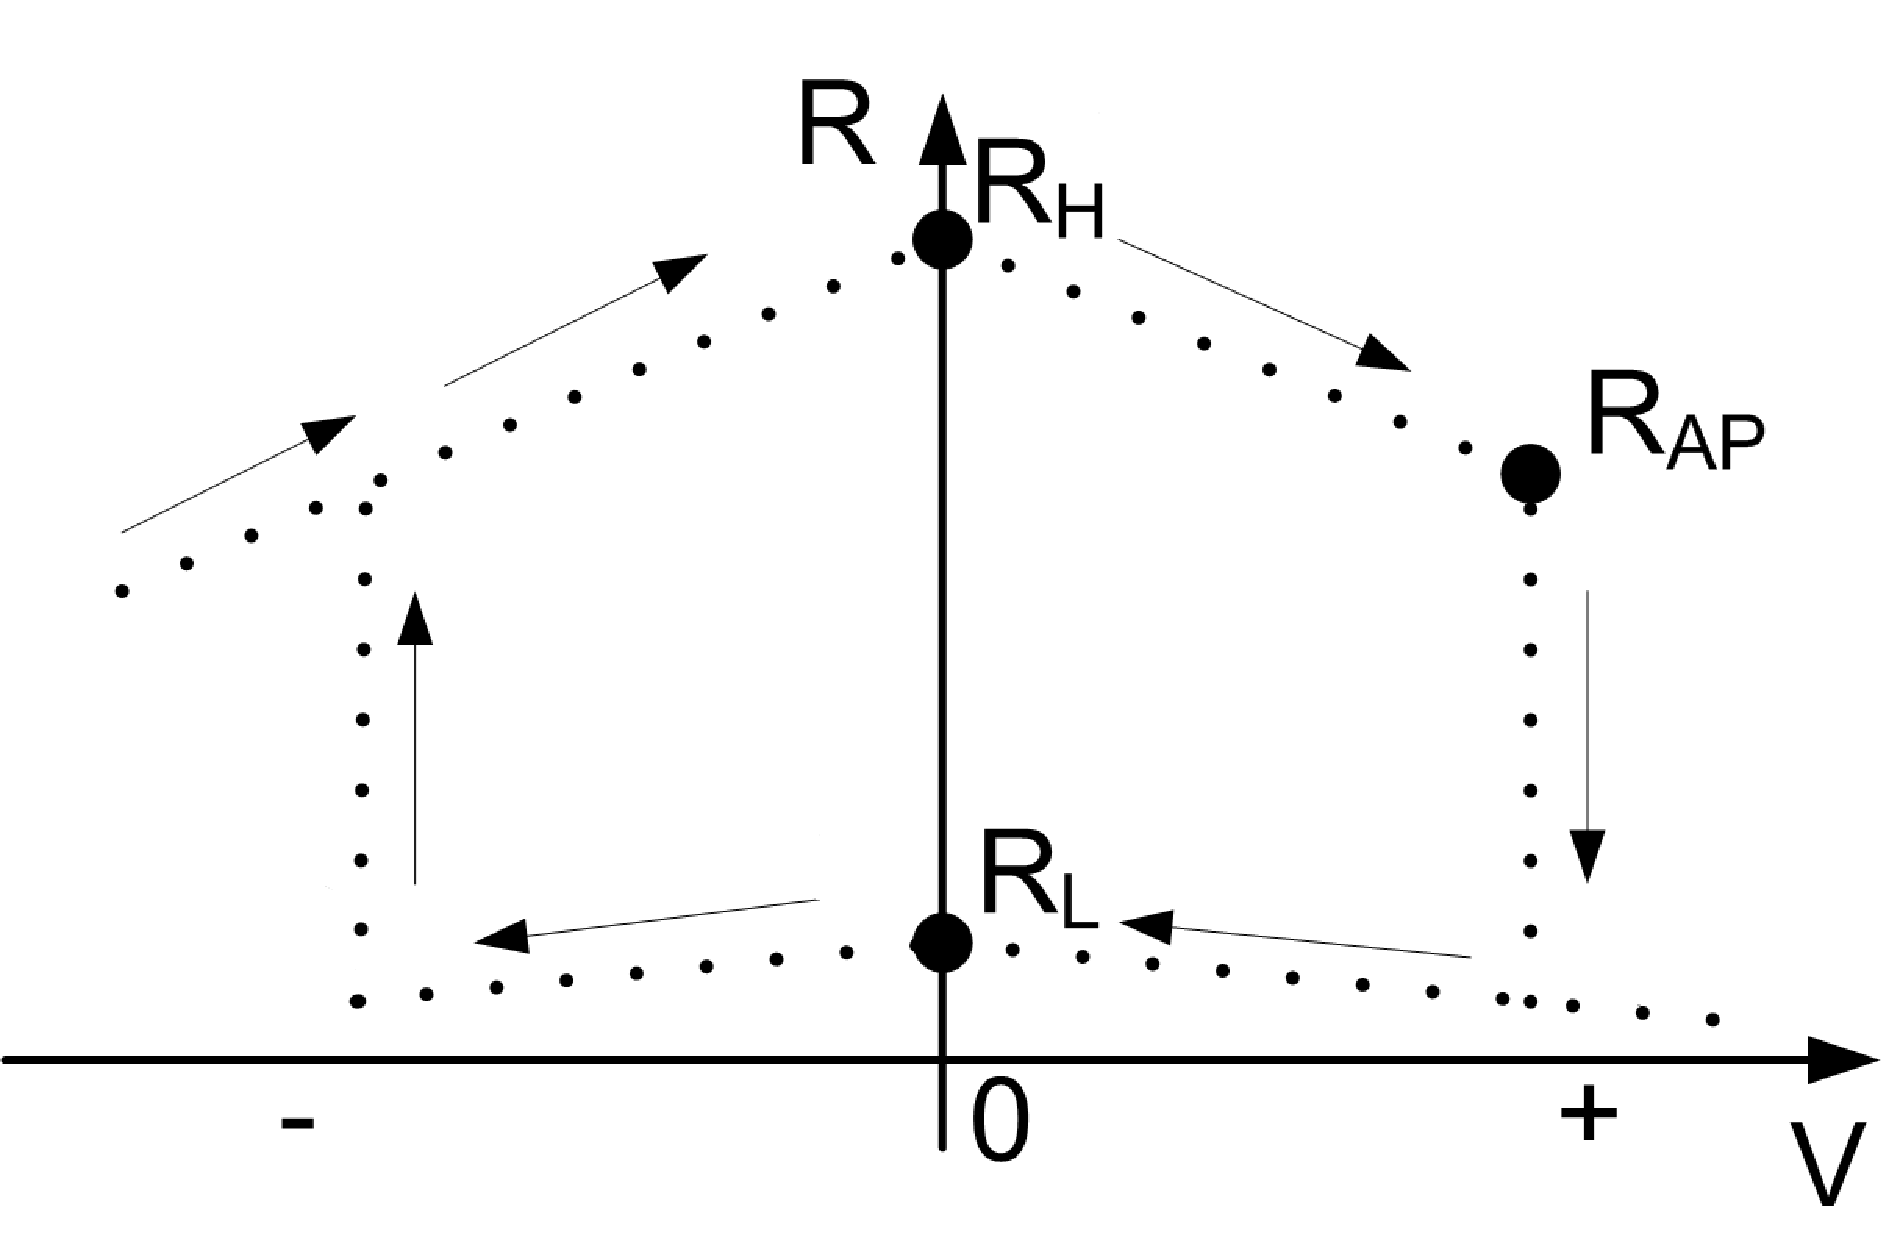
\includegraphics[width=0.45\textwidth]{./figure/RIcurve.pdf}
\caption{The static R-I curve of MgO-based MTJ.}\label{mtj-RI}
\end{wrapfigure}

Different from previous self-reference schemes, we propose a \textbf{\textit{non-destructive self-reference}} approach based on the special R-I characteristic of MgO-based MTJ's. As we can see in Figure~\ref{mtj-RI}, the MTJ current dependence of the high and the low resistance states are quite different: the current roll-off slope of high resistance is much steeper than that of low resistance. Therefore, we can sample the stored value of an MTJ twice by using two read currents $I_{R1}$ and $I_{R2}$ and compare the resistance difference $dR=R1-R2$. Obviously $dR_H$ when the MTJ is at the high resistance state should be pretty big, while $dR_L$ when the MTJ is at the low resistance state is close to `0'.

\paragraph{Preliminary results:} The scheme of our proposed nondestructive self-reference scheme is shown in Figure~\ref{self-ref}. A switch transistor SLT1 is connected to BL as well as the corresponding voltage storage element C1. The other switch transistor SLT2 is connected to a voltage divider. The top connect point of C1 ($V_{BL1}$) and the output of the voltage divider ($V_{BL2O}$) are connected to the two inputs of a voltage sense amplifier, respectively. The voltage divider is used to eliminate the impact of difference between two read currents $I_{R1}$ and $I_{R2}$. The operation of our proposed nondestructive self-reference scheme includes three steps: (1) First read: A read current $I_{R1}$ is applied and incurs the corresponding $V_{BL1}$, which is stored in C1. (2) Second read: Another read current $I_{R2}$ is applied and incurs $V_{BL2}$. $V_{BL2}$ goes through voltage divider and generate $V_{BL2O}$. (3) Sensing: $V_{BL1}$ and $V_{BL2O}$ are compared by the voltage sense amplifier. If $V_{BL1}$ is significantly larger than $V_{BL2O}$, the original value of STT-RAM bit is ��1�� (high resistance state). Otherwise, the original value of STT-RAM bit is ��0�� (low resistance state).

\begin{wrapfigure}{r}{0.5\textwidth}\centering \centering
\vspace{-18pt}
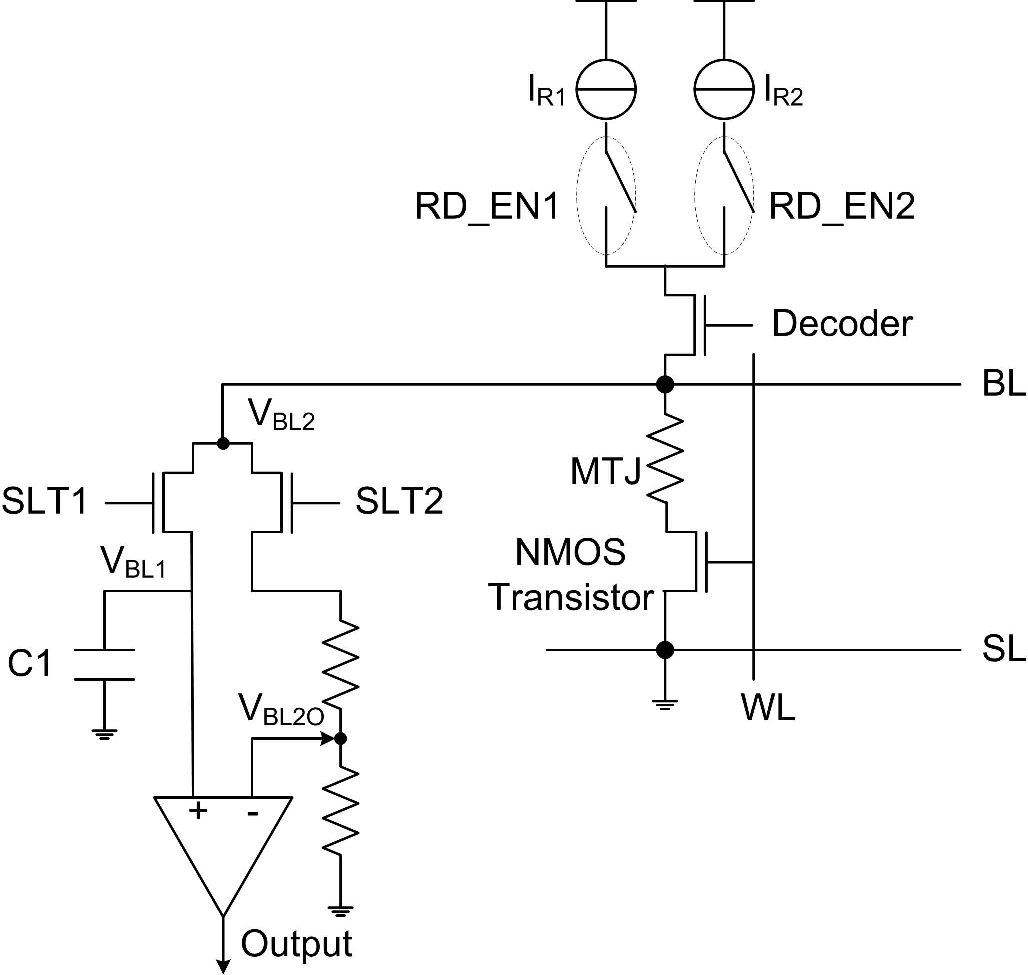
\includegraphics[width=0.5\textwidth]{./figure/self-ref.pdf}
\caption{Nondestructive self-reference sensing scheme for STT-RAM.}\label{self-ref}
\end{wrapfigure}

Compared to the conventional self-reference scheme\cite{Tanizaki06,Jeong03,Li:147723}, the proposed scheme can provide much faster read speed by eliminating two write steps (erase and write-back), which make it possible to utilize STT-RAM on-chip as well as satisfy the performance requirement. The reliability of STT-RAM is improved too by eliminating the unnecessary disturbances (writing) during read operations. However, to fully realize this approach, there are still some circuit issues to be solved. For example, the sensing margin of the proposed scheme is bigger than the one of conventional STT-RAM read scheme, but smaller the one of the ``destructive'' self-reference. So what type of sense-amplifier design is the best with the consideration on both accuracy and speed requirement? How to reduce the impact on overall area of peripheral circuitry? Will the traditional SRAM-liked memory array structure is good enough or some novel structure could be more beneficial? Furthermore, how will process variations, including both MTJ and CMOS processes, affect the proposed read scheme? In this project, we will address these circuit issues from both device and circuit point of views and explore the solutions.

\begin{comment}
The small $\Delta$R and the large $\sigma$ may lead to the errant detection of stored value: when \textit{R}$_L$ (\textit{R}$_H$) is higher (lower) than \textit{R}$_{ref}$ (=${\frac{R_L+R_H}{2}}$ ideally), the value stored in MTJ is always detected as ``1'' (``0'') (See Figure~\ref{mtj-distribution})~\cite{Li09}. As memory array size increases and process variation shows more impact, the traditional technologies, such as redundancy and ECC technologies, could not fully recover the yield required at production level.
\begin{figure}\centering
\includegraphics[width=0.60\textwidth]{./figure/mtj-distribution.png}
\caption{MTJ resistance distribution incurs read failure.}\label{mtj-distribution}
\end{figure}

To reduce read failures and improve chip yield, we propose a self-reference methodology in STT-RAM design. The idea is to compare the stored data in a memory cell with a reference value written to the same cell. By limiting the comparison within one single STT-RAM cell, the impact of MTJ resistance variation can be avoided. Previously some self-reference schemes were used in toggle-mode MRAM design~\cite{Tanizaki06,Jeong03}. We also successfully utilized it in STT-RAM design~\cite{Li:147723}. These schemes are all ``destructive'' because the original value in memory cell is wiped out when writing the reference value into MTJ, and has to be recovered at the end of the read operation. Obviously it prolongs read latency and introduces reliability issue. Based on the theory we proposed in~\cite{Chen:147727}, \textbf{\textit{non-destructive self-reference}} approach could be a better solution since the original data is not disturbed during read operations. However, there are some uncertainties to realize this approach. For example, does it need a new sense-amplifier (SA) with high resolution? How accurate should it be? If new SA and write driver are needed, how to reduce the impact on overall area of peripheral circuitry? Will SRAM-liked memory array is good enough or some novel structure could be more beneficial? In this proposal we will investigate these circuit issues and exploring the solutions. Our target is to minimize the effect of process variation and to improve read speed.

The most serious problem for STT-RAM is high write current. At 90nm technology node and with 15ns write pulse width, the required magnitude of writing current to switch MTJ resistance is at least 300$\mu$A~\cite{Wang08}. The high write current causes several main issues. (i) Reliability gets worse due to the electromigration-induced damage on the metal wires. (ii) High peak current and power consumption constrain the write bandwidth. (iii) The scalability is limited because the selection transistor in memory cell needs to be large enough to provide the writing current to MTJ.

A number of material solutions have been proposed to reduce the write current, such as adding perpendicular anisotropy~\cite{Sun:20050104101} and/or introducing surface anti-ferromagnetic coupled (AFC) magnetic layer in MTJ structure~\cite{Beech00}. We will concentrate on device and circuit techniques to help out. On possible solution is overdriving the gate of the selection transistor to increase $V_{GS}$, and consequently enhance its driving ability~\cite{Li09}. However, overdriving cannot write ``0'' and ``1'' simultaneously because they have different gate voltage requirement. Therefore, system need to support two-step writing or program/erase operations. A bootstrapped driver can also help by providing higher $V_{GS}$~\cite{Li:426098}or $V_{DS}$ of the select transistor in a short pulse. In the case of unsuccessful writing, a verification and recovery scheme might be needed. To relieve the burden of power supply, evenly distribute the bits in one write operations on floorplan is also an interesting solution. How to build the corresponding memory hierarchical structure and how it will impact memory performance on architecture level will be part of our research work.
\end{comment}


\subsubsection{Task C-2.2: PCRAM -- endurance enhancement}

PCRAM exploits the large resistance contrast between the amorphous and crystalline states in phase-change materials~\cite{Raoux08}. The resistance difference could be four or five orders sometime. Given such a large resistance contrast, the difference in read current is read current is more than sufficient for binary storage and even MLC (multi-level cell) operation~\cite{Raoux08}.

The most stringent requirement to prevent PCRAM from production is endurance. While READ endurance is not likely a problem, the best reported WRITE endurance for PCRAM is only 10$^9$ based on a survey of PCRAM device and circuit prototypes published within the last five years~\cite{Lee09}. Besides the improvement on material, we could also help out in circuit design level. From circuit design point of view, we could also help out in many ways and this will be our objective in the proposal.

One possible solution is smoothing the driving current during write operations and avoiding the overshot on phase change materials. Here, how to design a write driver to provide a sleek but fast ramp-up curve is the tricky part. We should also reduce memory access time, especially for SET/RESET operations, because endurance failure is directly related to the duration of energy applied on phase change material. Obviously an accurate self-timing control scheme is required, which can stop providing current to memory cells once detecting successful SET/RESET operations. Another interesting method could be lowering the voltage on phase change material to meet only the minimal SET/RESET requirements because the failure increases exponentially when energy increases. Furthermore, for some applications that non-volatility is not a requirement (i.e. directly replace SRAM with PCRAM), we can trade data retention with endurance by further reducing the energy pulse. Of course, the statically or dynamically fixing by using redundancy and ECC will keep useful. However, will the more complex ECC algorithms or bit-level redundancy be needed? We will investigate it in the proposal.

%Some architectural level solutions have been proposed, such as early write termination~\cite{Zhou09} or partial writes~\cite{Lee09}.

%Density is always a concern in all memory designs. PCRAM is no exception. That's why diode-switch PCRAM is preferable~\cite{Zhang07,Rajendran07}. However, the area overhead of memory peripheral circuits could be a potential issue for high-density diode-switch PCRAM design. Although a diode-based row/column decoder is proposed in~\cite{Li09}, the decoder encounters high-power consumption due to the directly paths from VDD to VSS through diodes.

\subsubsection{Task C-2.3: RRAM -- density improvement}
\label{C2.3-RRAM}

RRAM is expected to replace NAND Flash memory as main storage in near future~\cite{ITRS07}. Hence, increasing memory density becomes the ultimate goal in RRAM design. Usually an NMOS transistor is used as selection device in a random access memory cell (\emph{e.g.} DRAM and MRAM) by connecting it in series with the data storage element. Such a cell structure needs three sets of terminals -- word line (WL), bit line (BL) and source line (SL). The routing requirement and design rules determine that the minimal cell size is 12$F^2$~\cite{Li09}, which is too big to be tolerant in RRAM design. Here, $F$ represents the technology feature size. Theoretically, the smallest memory cell is 4$F^2$, which has only two terminals -- one is horizonal and another is vertical. The storage element is built at the cross-point of two metal wires. Hence, this is called cross-point structure. %(See Figure~\ref{RRAM1}(a))
Moreover, the cross-point structure can grow in third dimension, which is called intra-die stacking. %as shown in Figure~\ref{RRAM1}(b)
The memory storage cell is located in between any two adjacent metal layers which are used as interconnects. Within the same die size, the multiple memory layers further improve the memory density. Hence, cross-point structure is widely investigated in RRAM design.

\begin{comment}
\begin{figure}\centering
\includegraphics[width=0.60\textwidth]{./figure/HL-RRAM1.png}
\caption{RRAM memory array. (a) Cross-point structure; (b) Intra-die structure.}\label{RRAM1}
\end{figure}
\end{comment}

From design point of view, RRAM technologies can be divided into two operation types: unipolar switching and bipolar switching. Unipolar operation executes the programming/erasing by using short and long pulse, or by using high and low voltage with the same voltage polarity. Usually a diode is served as selection device (1D1R). The data in bipolar switching RRAM can be changed by short voltage/current pulses with opposite voltage polarity. For such memory structures, non-ohmic device (NOD)~\cite{Yan4430255} is used to provide two-direction driving current as well as support process integration of cross-point structure. We call it as 1NOD-1R (See Figure~\ref{RRAM2}).

However, 1D1R and 1NOD-1R cell structures are facing on some design difficulties due to process limitation. Conceptually, NOD can be understood as two parallel connected diodes. Ideally, it turns on only when the voltage drop between the two terminals exceeds its threshold. However, the I-V characteristic curve of real device could be quite different.
%(See Figure~\ref{NOD}. Please note that the curves are not in the same scale.)~\cite{Yan4430255}.
This results in sneak path which has three or more cells in series as shown in Figure~\ref{RRAM2}(b). The sneak current can introduce disturbance on unintended cells during read, write and erase operations. Therefore, diode (P-N or Schottky) is more favorable as a selective element for RRAM array and intra-die stacking. However, it is extremely difficult to achieve the high quality diode with large $I_{on}$/$I_{off}$ ratio (large forward current $I_{on}$ and extremely small reverse current $I_{off}$) by using temperature limited BEOL (back end of line) process ($<400 ^{\circ}C$)~\cite{Sun:147791}.

\begin{figure}\centering
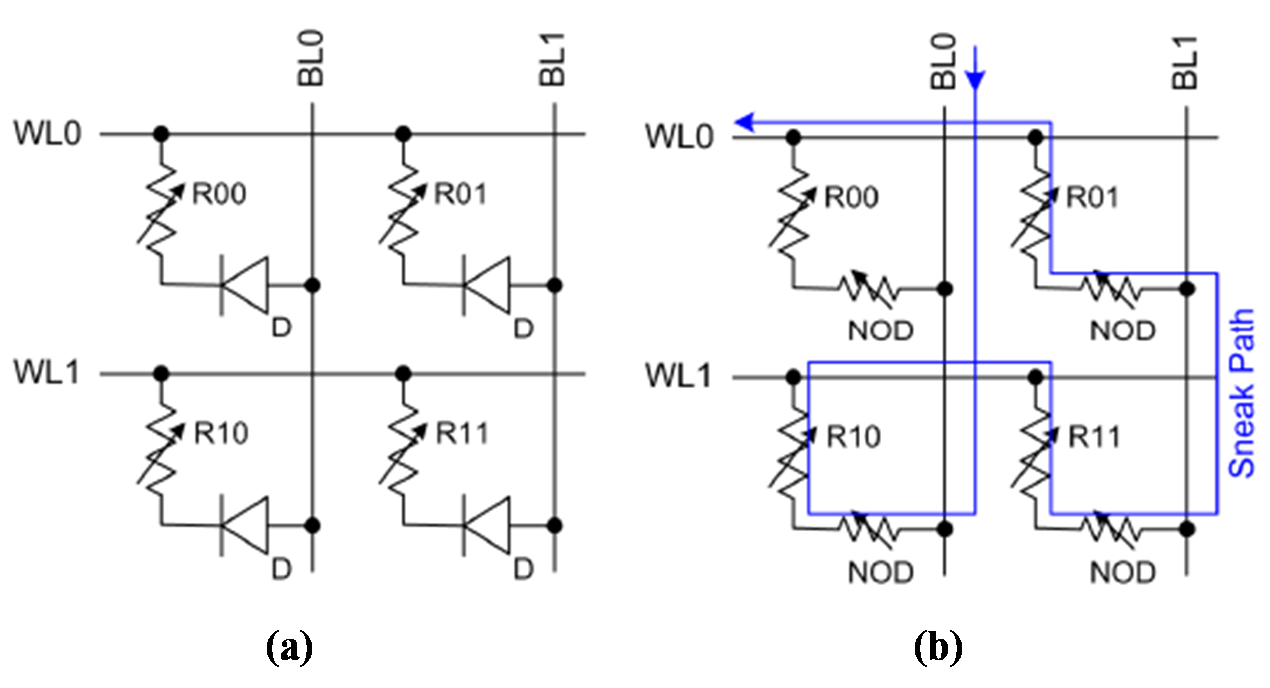
\includegraphics[width=0.50\textwidth]{./figure/HL-RRAM2.png}
\caption{RRAM memory cell scheme. (a) 1D1R; (b) 1NOD-1R.}\label{RRAM2}
\end{figure}

\begin{comment}
\begin{wrapfigure}{r}{0.40\textwidth}\centering \centering
\vspace{-18pt}
\includegraphics[width=0.40\textwidth]{./figure/HL-NOD.png}
\caption{NOD IV characteristic curve.}\label{NOD}
\end{wrapfigure}
\end{comment}

\paragraph{Using bipolar PMC as the selective element.} We propose to bipolar resistive switching devices as the selection device. Programmable-metallization-cell (PMC) could be a good candidate.
PMC ~\cite{Kozicki05} is a promising bipolar RRAM technology, which is composed of two solid metal electrodes -- relatively, one is inert and the other is electrochemically active. Between the two electrodes locates a thin electrolyte film. When a negative bias is applied to the inert electrode in programming operation (SET), metal ions in the electrolyte together with those flew from the positive active electrode can be reduced by the inert electrode. As a result, the metal ions form a small metallic ``nanowire'' between the two electrodes, which produces a low resistance. In erasing operation (RESET), a positive bias is applied on the inert electrode. Metal ions migrate back into the electrolyte and eventually to the negatively-charged active electrode. The ``nanowire'' is broken and the resistance increase back. The I-V curve is illustrated in Figure~\ref{PMC}(a). A higher voltage is required in RESET operation ($V_{r}$)than the one in SET operation ($V_{s}).

\begin{figure}\centering
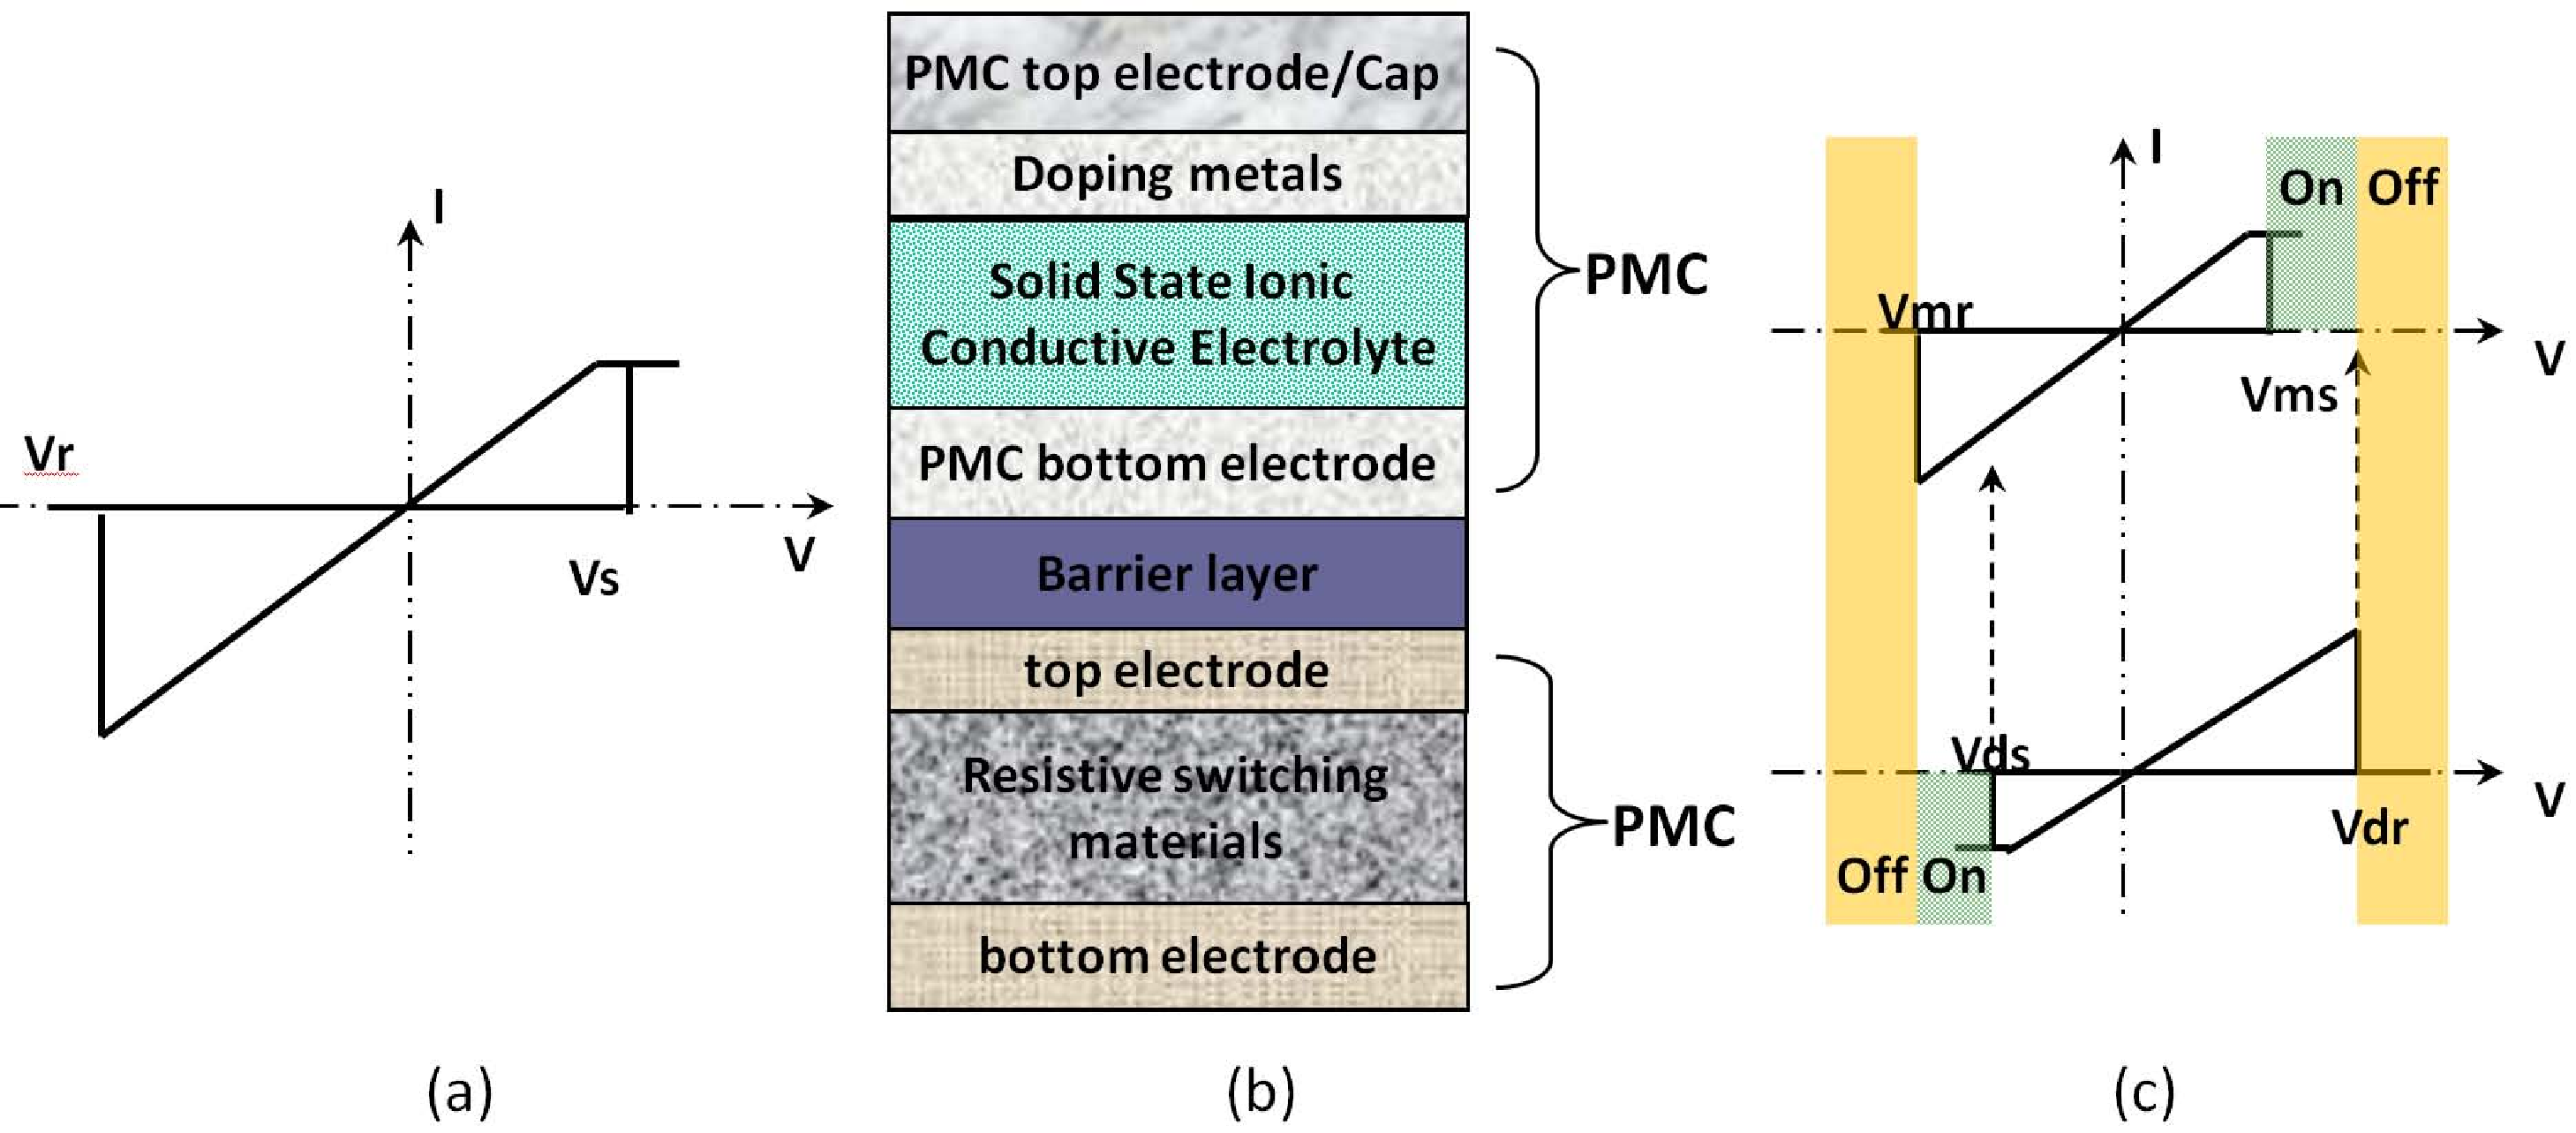
\includegraphics[width=0.75\textwidth]{./figure/PMC.png}
\caption{(a) I-V curve of PMC; (b) The proposed double cell configuration based on PMC technology; (c) I-V curves of the two back-to-back PMC devices shown in (b).}\label{PMC}
\end{figure}

\paragraph{Preliminary results:} Figure~\ref{PMC}(b) demonstrates a double cell configuration built by stacking two PMC's back to back with a barrier layer in between. In this structure, the PMC with active electrode on top is used as data storage (RRAM), while the main function of the PMC with active electrode at bottom is the selective device. This cell structure has been successfully demonstrated in process~\cite{Sun:147791}. Since PMC technology itself is compatible to CMOS process, the integration of the proposed structure is friendly to CMOS technology too. 

The operations can be explained by using the corresponding I-V curves of the two PMC devices shown in Figure~\ref{PMC}(c). Here, the top and bottom I-V curves are for the memory and selection devices, respectively. We can see that when the voltage drop cross the RRAM cell exceed $V_{r}$, the RRAM cell is ``off'' because either PMC1 or PMC2 are in high resistance state.
\begin{itemize}
  \item SET operation: First, a negative bias in between $-V_{ds}$ and $-V_{mr}$ is applied to turn on the switch; Then a positive voltage higher than $V_{ms}$ but smaller than $V_{dr}$is used to program memory. After data is successfully written to the cell, further increase voltage to higher than $V_{dr}$ in order to turn off the switch.
  \item RESET operation: Apply a negative bias lower than $-V_{mr}$, it will first turn on the switch and than reset the memory cell. In such a situation, there is no way to turn off the switch.  But there is no leakage path either due to the high resistance of the memory.
  \item READ operation: Like SET and RESET, the switch needs to be turned on first by applying a negative bias in between $-V_{ds}$ and $-V_{mr}$. Then a small current can be used to read memory cell resistance state.  At the end of the read operation, the switch is required to turned off or keep it on when memory is in low or high resistance state, respectively.
\end{itemize}

Compared to diode or NOD, PMC based switch has two advantages -- bipolar switching and large $I_{on}$/$I_{off}$ ratio. Hence, the proposed scheme could be used in bipolar switching RRAM design with minimized sneak current. Although we have investigate the feasibility based on theoretical analysis, there are still a lot of unsolved issues. For example, how to control timing and applied voltage? What kind of peripheral circuitry floorplan will be optimal for the proposed RRAM design? And again, how will process variations affect the proposed RRAM scheme? In this project, we will address these circuit issues from both device and circuit point of views and explore the solutions.
